\documentclass[11pt]{article}
\usepackage{geometry}
\geometry{a4paper, left=20mm, top=20mm}
\usepackage{amsmath}
\usepackage{graphicx}
\usepackage{hyperref}
\usepackage[T1]{fontenc}
\usepackage{polski}
\usepackage[utf8]{inputenc}

\usepackage{xcolor}

\title{Aplikacja książka kucharska}
\author{Mikołaj Kubik}

\begin{document}
\maketitle
\section{Wstęp}
Celem projektu było stworzenie aplikacji webowej, będącej publiczną książką kucharską. Użytkownicy mogą dodawać nowe składniki
oraz tworzyć z nich przepisy a także dodawać komentarze do istniejących przepisów. W bazie danych przechowywane są wartości 
odżywcze poszczególnych składników, dzięki czemu użytkownik może lepiej dopasować dany przepis do swoich preferencji żywieniowych.

\section{Architektura techniczna}
\subsection{Wykorzystane narzędzia}
\begin{itemize}
    \item Docker
    \item Django
    \item React
    \item MS SQL
\end{itemize}
\subsection{Baza danych}
\subsubsection{Diagram bazy danych}
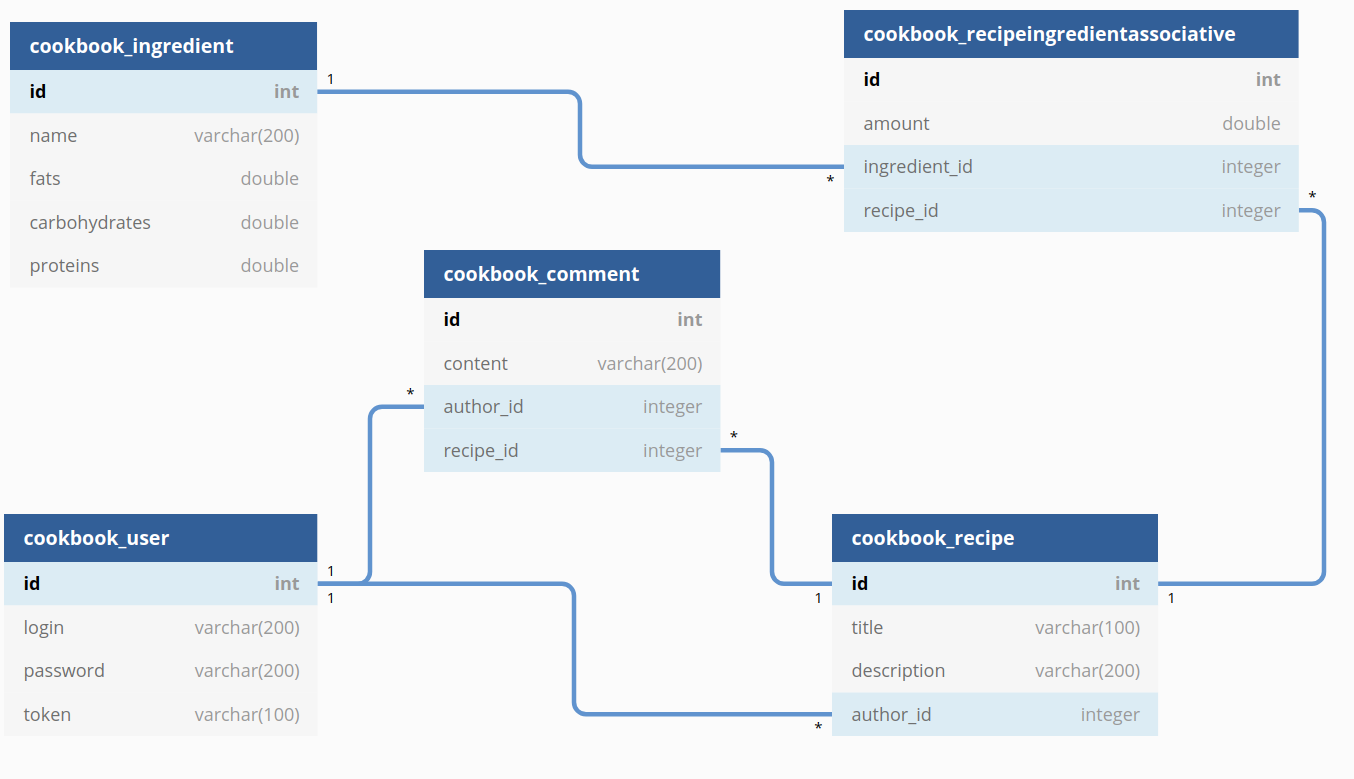
\includegraphics[width=15.5cm]{db_diagram.png}
\subsubsection{Skrypt tworzący bazę danych}

\section{Strona serwerowa}

\section{Dokumentacja aplikacji}
\subsection{Dodawanie składników}
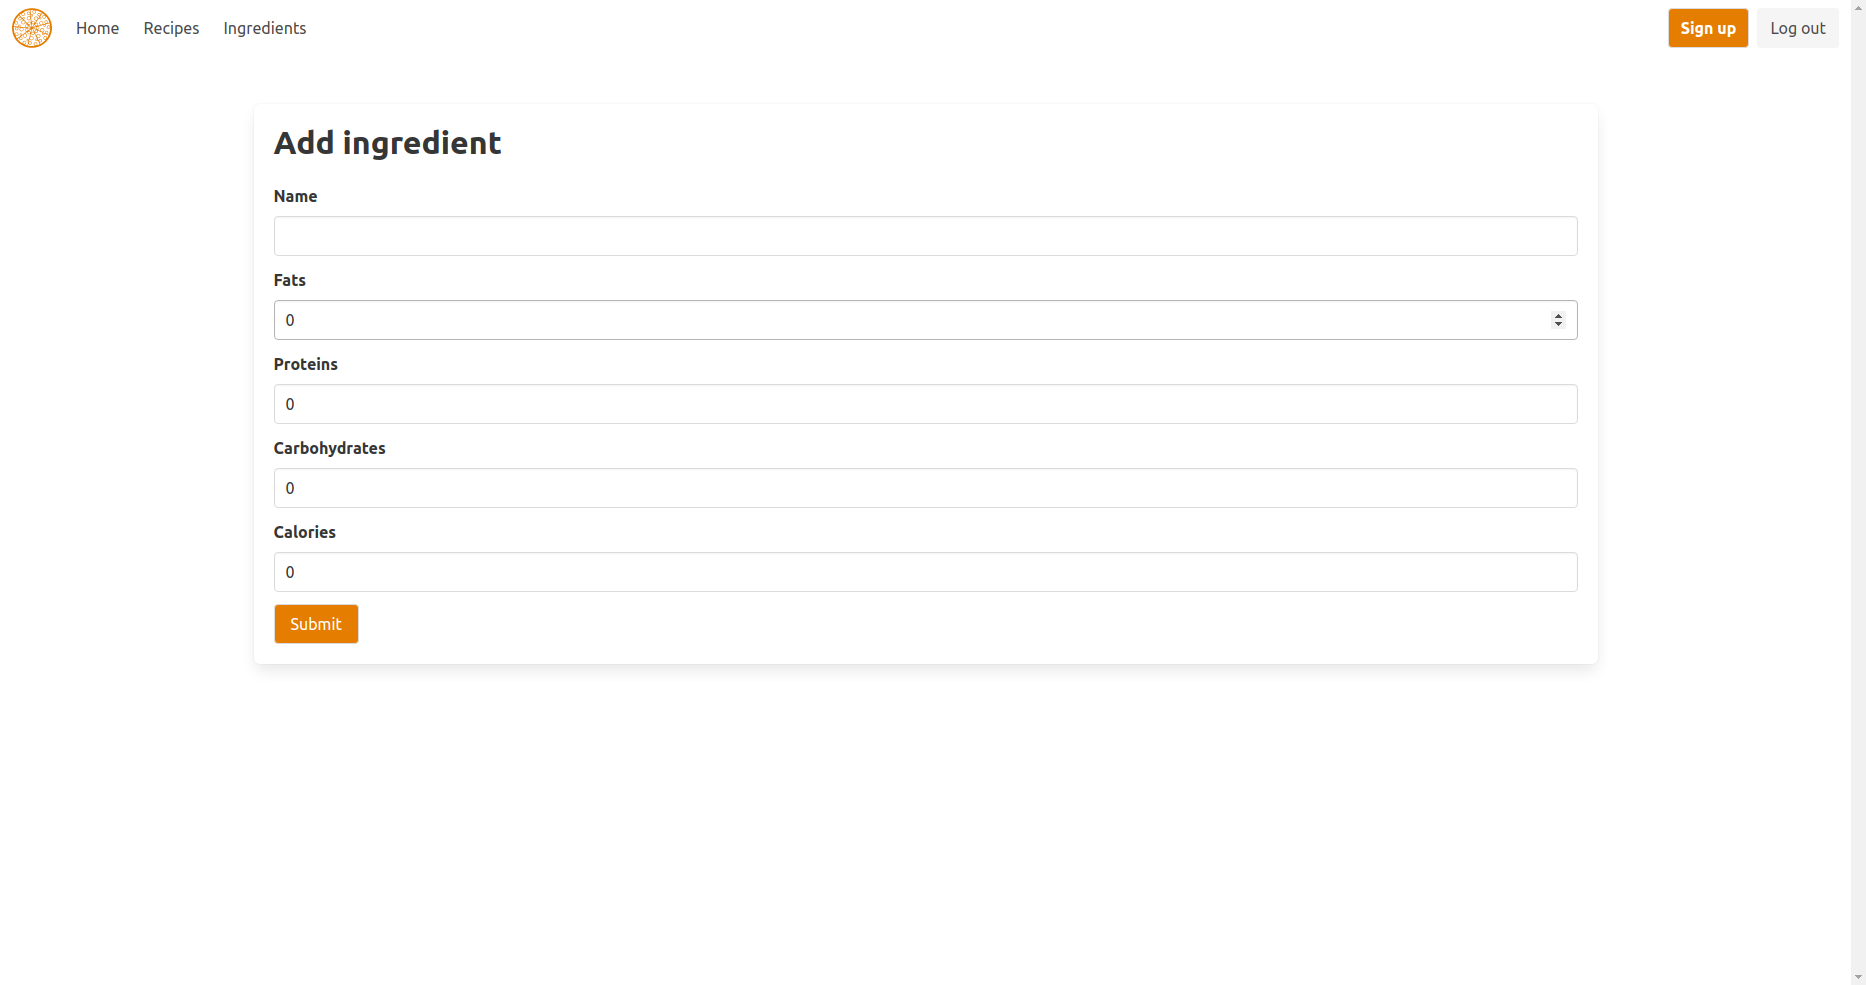
\includegraphics[width=15.5cm]{add_ingredient.png}
\subsection{Wyświetlanie listy składników}
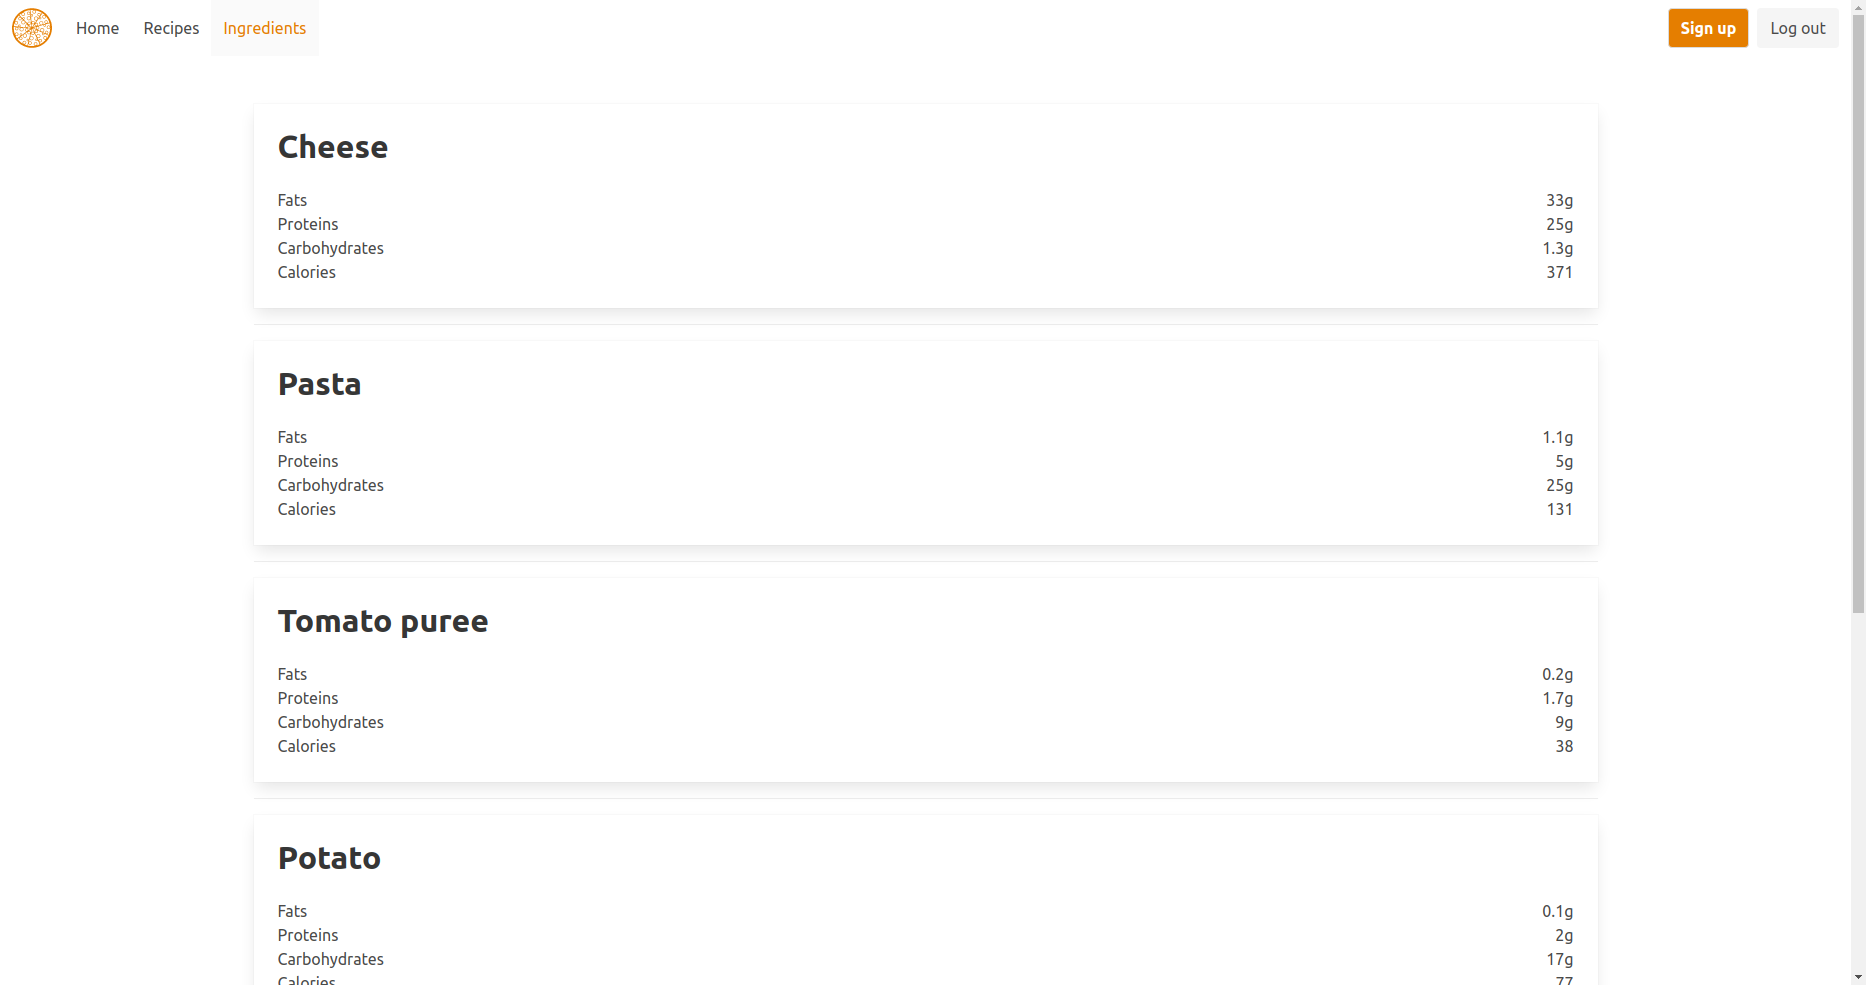
\includegraphics[width=15.5cm]{ingredients_list.png}
\subsection{Dodawanie przepisu}
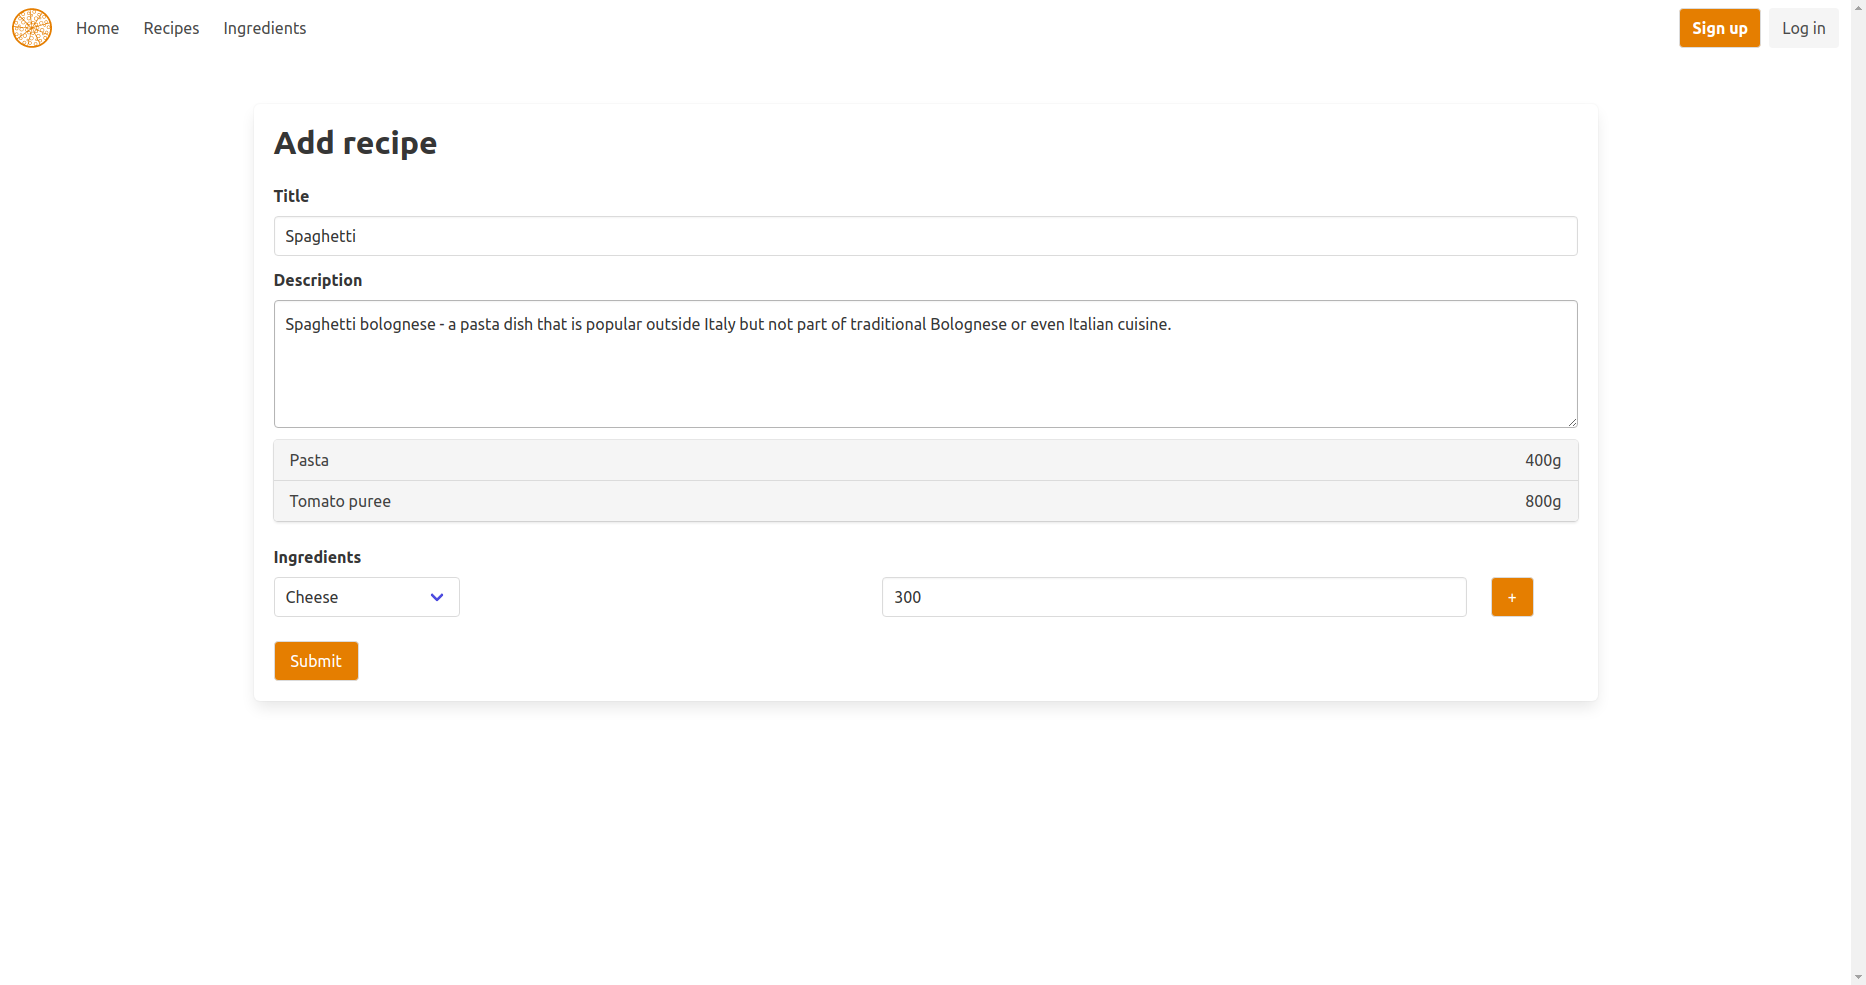
\includegraphics[width=15.5cm]{add_recipe.png}
\subsection{Wyświetlanie listy przepisów}
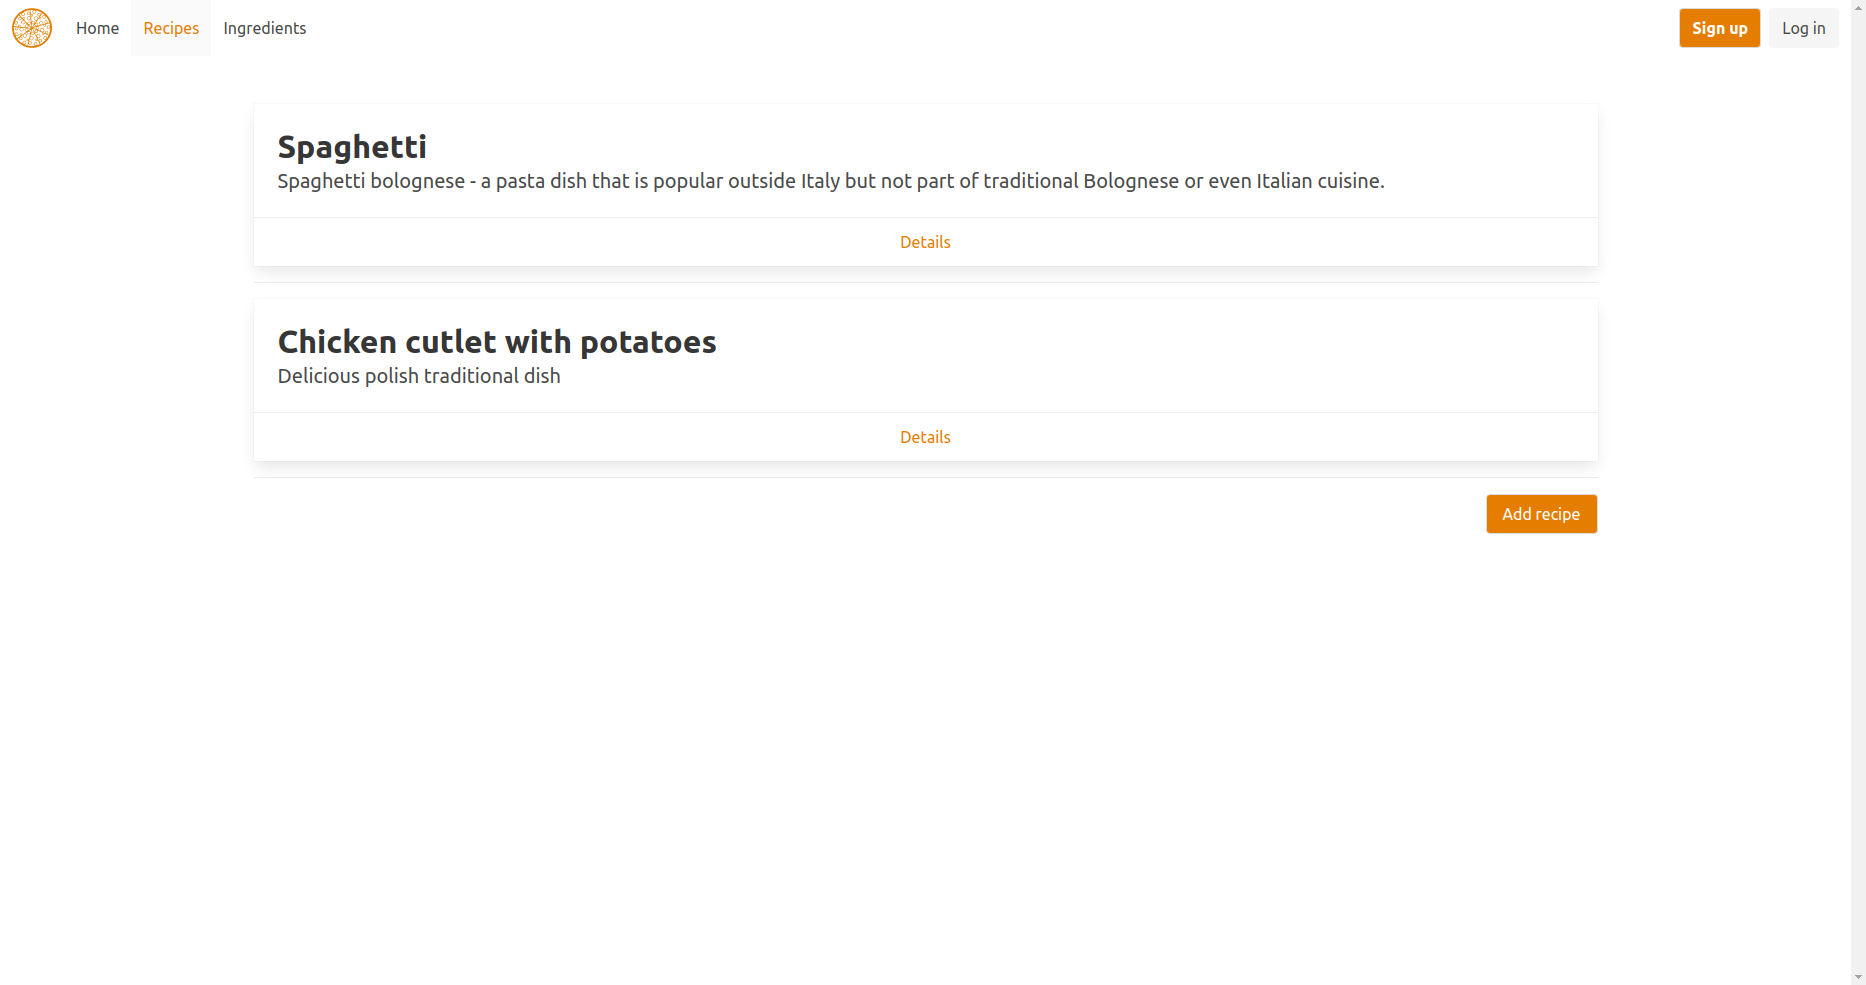
\includegraphics[width=15.5cm]{list_of_recipes.png}
\subsection{Wyświetlanie szczegółów przepisu}
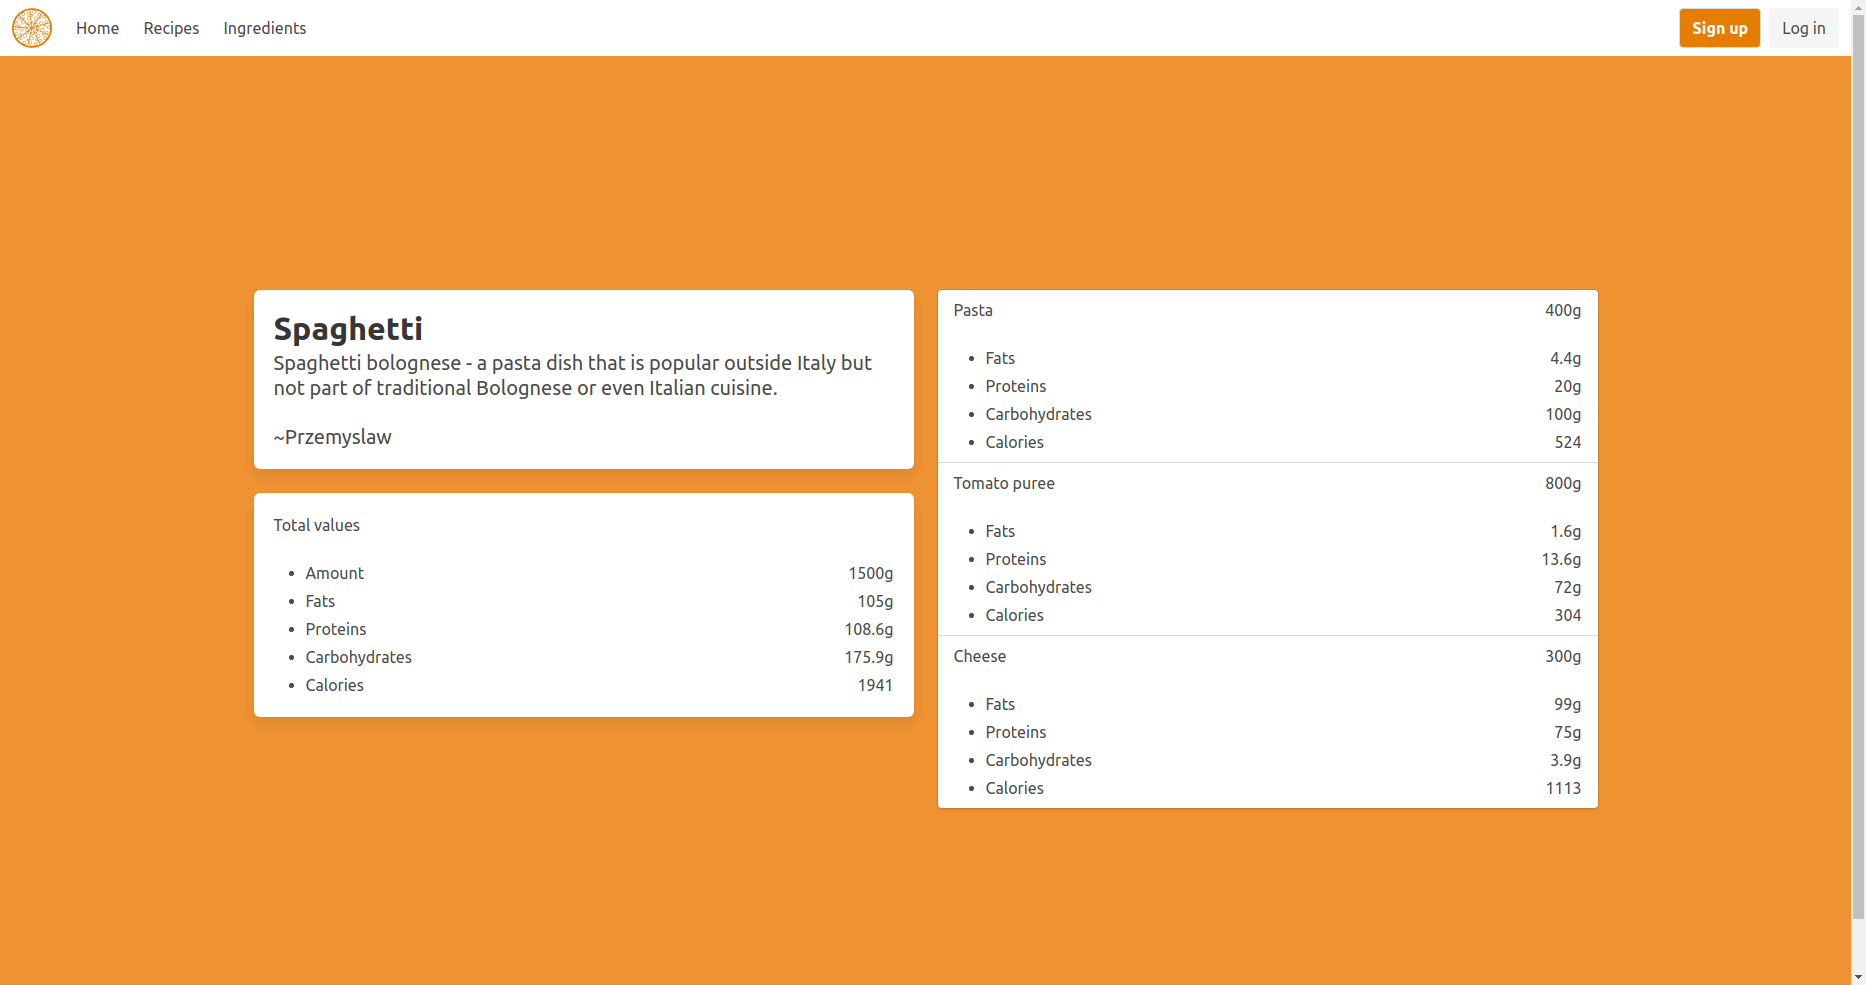
\includegraphics[width=15.5cm]{recipe_view.png}
\subsection{Wyświetlanie i dodawanie komentarzy do przepisu}
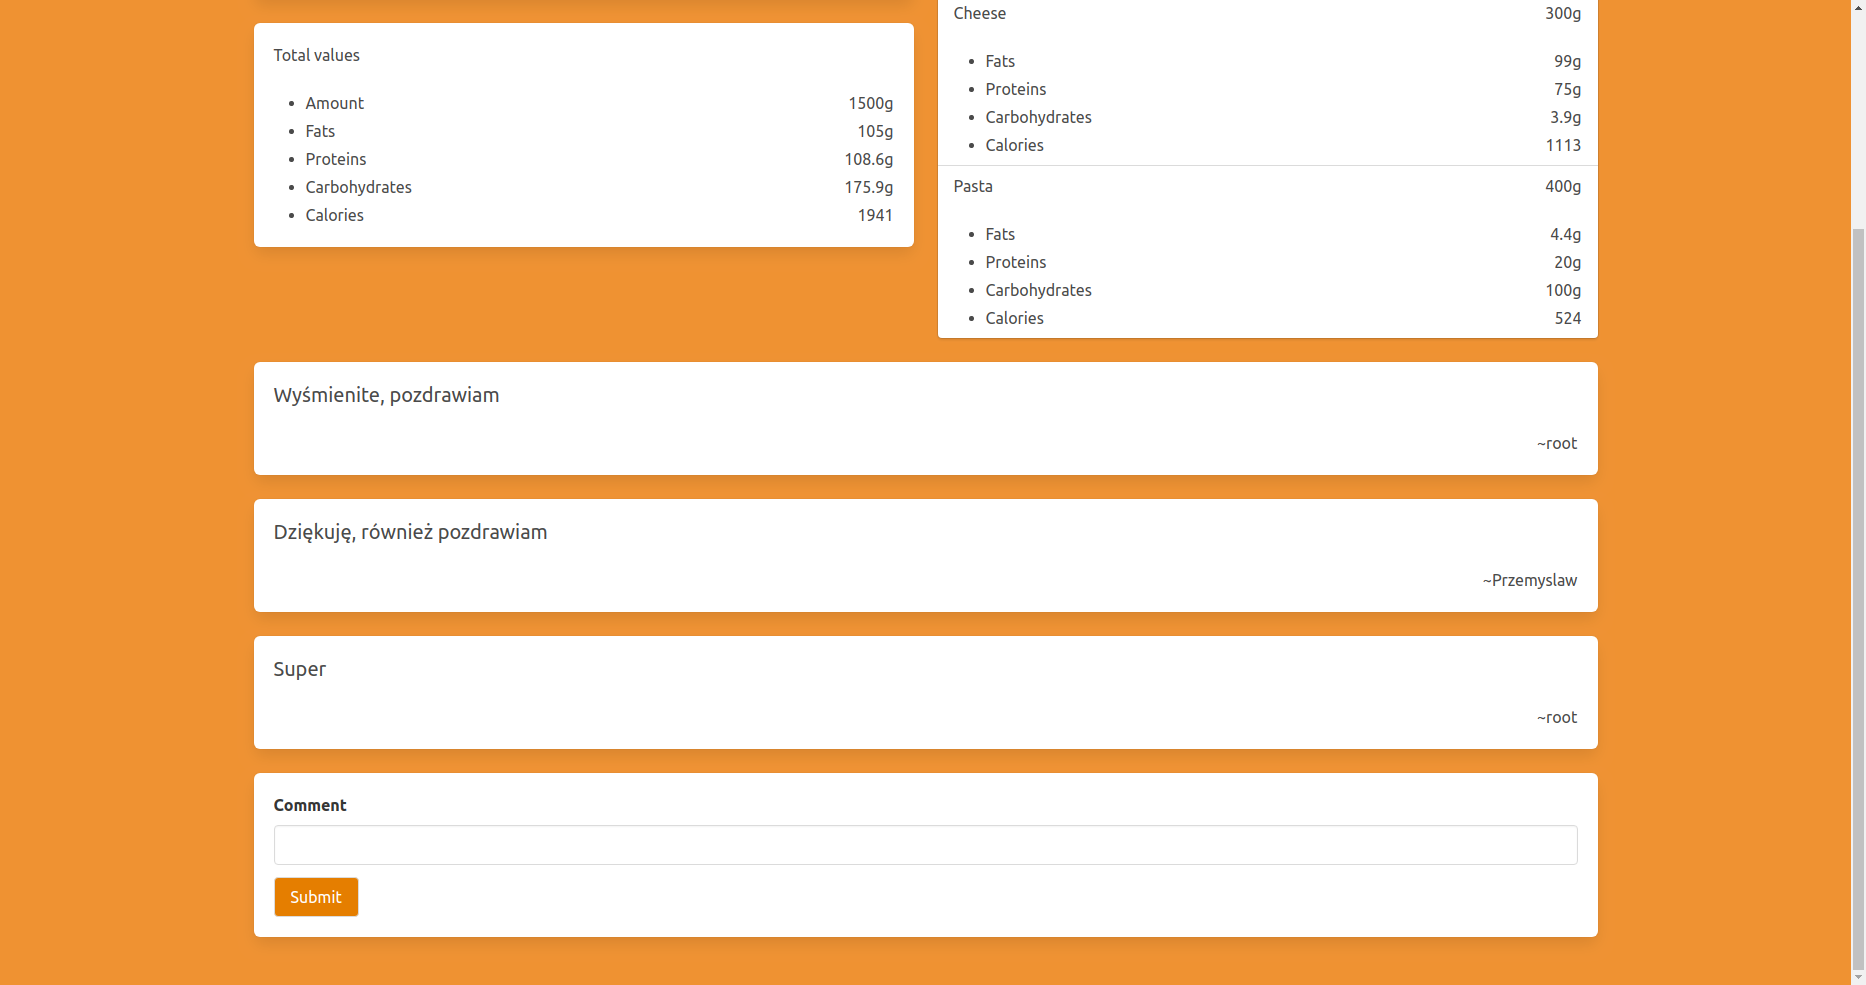
\includegraphics[width=15.5cm]{comments.png}

\section{Wnioski}
\section{Możliwości rozwoju}
\end{document}